In this section, I present a series of mini-experiments demonstrating the use
of timing-model in a MIDAS simulation. There is an unfortunate dearth of
experiments using the FRFCFS model, as there are still bugs in either BOOM,
MIDAS, or the model itself that cause many of the simulations to fail deep into
simulation.

\section{Latency-Bandwidth Pipe}

\begin{figure*}
\begin{subfigure}[t]{0.33\textwidth}
	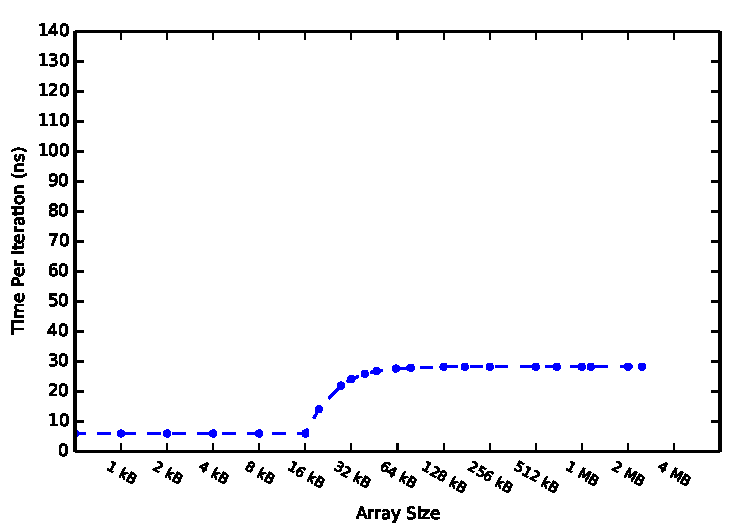
\includegraphics[width=\textwidth]{figures/ccbench_lat1.pdf}
	\caption{DRAM Latency = 1}
\end{subfigure}
\begin{subfigure}[t]{0.33\textwidth}
	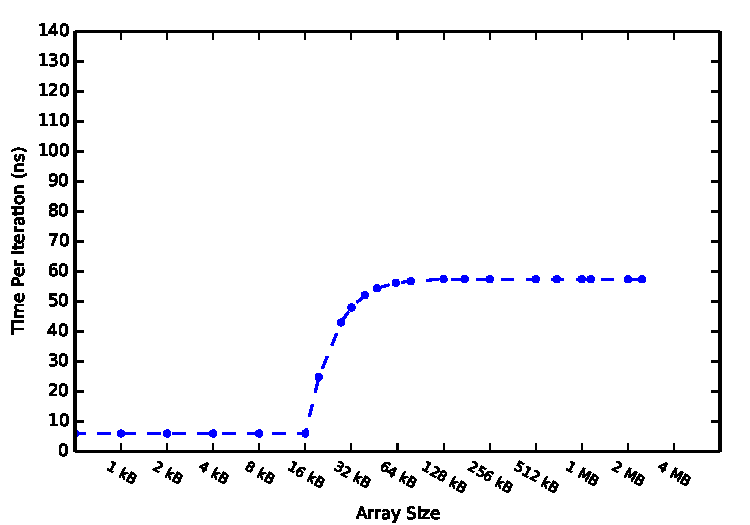
\includegraphics[width=\textwidth]{figures/ccbench_lat30.pdf}
	\caption{DRAM Latency = 30}
\end{subfigure}
\begin{subfigure}[t]{0.33\textwidth}
	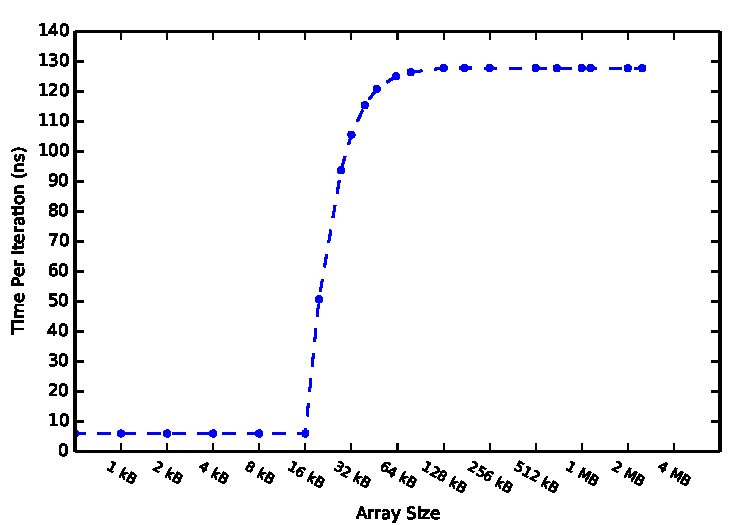
\includegraphics[width=\textwidth]{figures/ccbench_lat100.pdf}
	\caption{DRAM Latency = 100}
\end{subfigure}
\caption{Latency Validation}
\label{fig:lat_val}
\end{figure*}

Figure~\ref{fig:lat_val} shows the results of cache hierarchy tests in \textit{ccbench}
for BOOM-2w, assuming its frequency is 1GHz. We can see that the amount of
the time per iteration with arrays bigger than the cache size observed by the target system
increases by the delay of the off-chip memory as the DRAM latency increases.
In this case, 1 cycle is 1ns, and thus, the time per iteration with large arrays
increases by 30ns and 100ns as the DRAM latency increases by 30 cycles and 100 cycles,
respectively.

Figure~\ref{fig:gcc_ref} shows how CPI varies over time for \textit{403.gcc} with the reference
input set running on the Rocket processor. We first measure the performance with a
magic memory with a one-cycle latency to determine the maximum performance the Rocket processor can
achieve. Next, we increase the memory latency to 30 cycles and see how much the Rocket processor
slows down.

This experiment demonstrates that our simulation methodology enables ``what-if'' experiments
regarding memory parameter configurations for very long-running applications, which is
practically impossible with software simulators. Note that the dynamic instruction count for
\textit{403.gcc} with the reference input is 1.3 trillion (Table~\ref{tbl:spec_ref}). The
effective simulation rate is 29 MHz on the FPGA, whose operating frequency is 40 MHz. The
simulation slow-down is due to the communication overhead between the software components and the
FPGA-based simulator.

\begin{figure*}
	\centering
	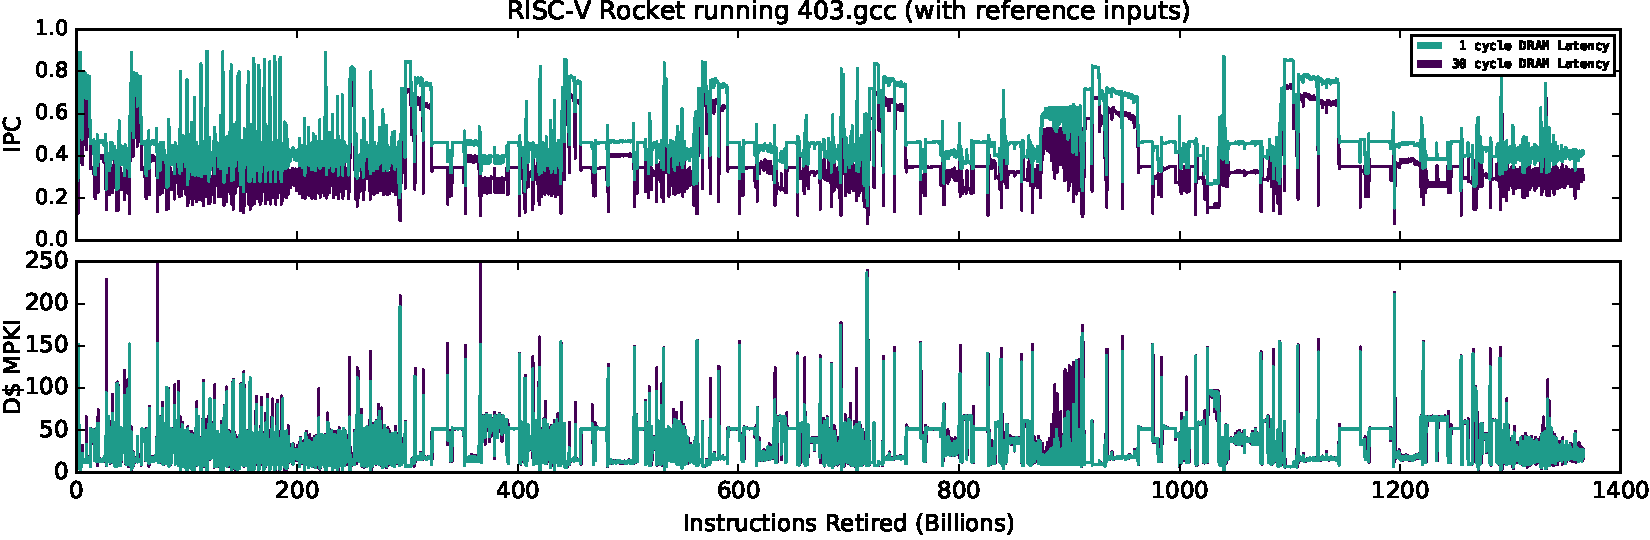
\includegraphics[width=0.95\textwidth]{figures/403-gcc-ref.pdf}
	\caption{CPI and D\$ MPKI for 403.gcc with the reference input running on the Rocket processor}
	\label{fig:gcc_ref}
\end{figure*}

\begin{figure}[t]
	\centering
	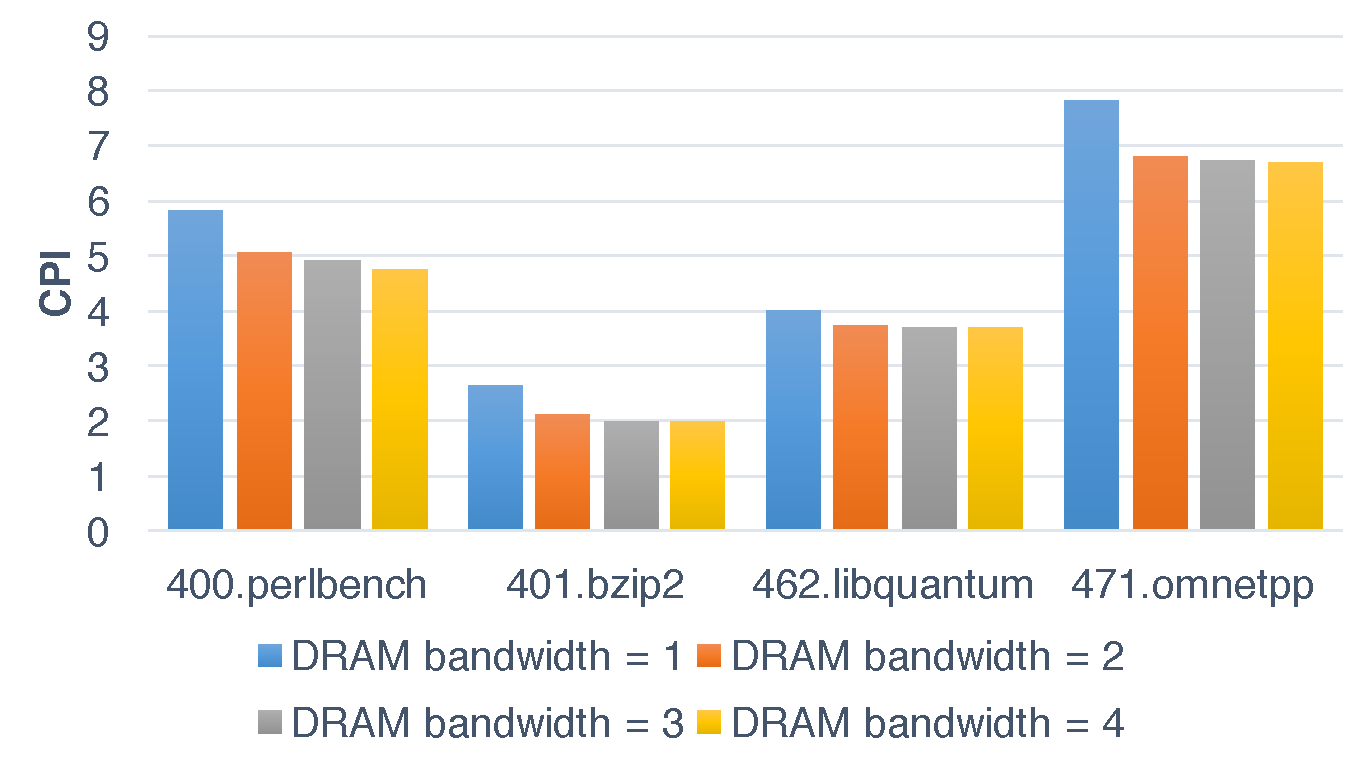
\includegraphics[width=0.8\columnwidth]{figures/boom-bw.pdf}
	\caption{CPIs for BOOM-2w with various bandwidths}
	\label{fig:bandwidths}
\end{figure}

Our next experiment highlights how various memory bandwidths affect the performance of
a superscalar out-of-order processor, assuming the DRAM latency is 100 cycles.
Figure~\ref{fig:bandwidths} shows CPIs for BOOM-2w with various bandwidth 
running \textit{401.bzip2}, \textit{462.libquantum}, and \textit{471.omnetpp}
with the test inputs.
We expect BOOM-2w to be able to issue more memory requests in flight than Rocket,
and thus, we believe memory bandwidth is an important parameter for this case study.
As seen in Figure~\ref{fig:bandwidths}, there is a significant performance
advantage when we increase the memory bandwidth from 1 to 2. However,
the performance benefits diminish as we increase the bandwidth further,
due to lack of memory-level parallelism in the benchmarks.

\section{Bank Conflict Model}

\begin{figure}[t]
	\centering
	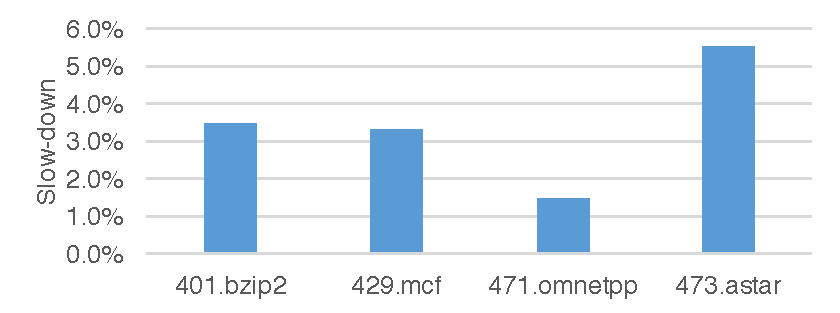
\includegraphics[width=0.8\columnwidth]{figures/boom-bc.pdf}
	\caption{Performance degradation from bank conflicts with 8 banks and a 20-cycle penalty}
	\label{fig:bank_conflict}
\end{figure}

Figure~\ref{fig:bank_conflict} shows how bank conflicts degrade the processor performance.
We run the benchmarks on BOOM-2w with a 8-bank DRAM by varying the bank conflict penalty 
from 1 cycle to 20 cycles. We can see the benchmarks suffer from performance degradation
due to bank conflicts as expected.

\section{FCFS MAS Model}

\begin{figure}[t]
		\centering
		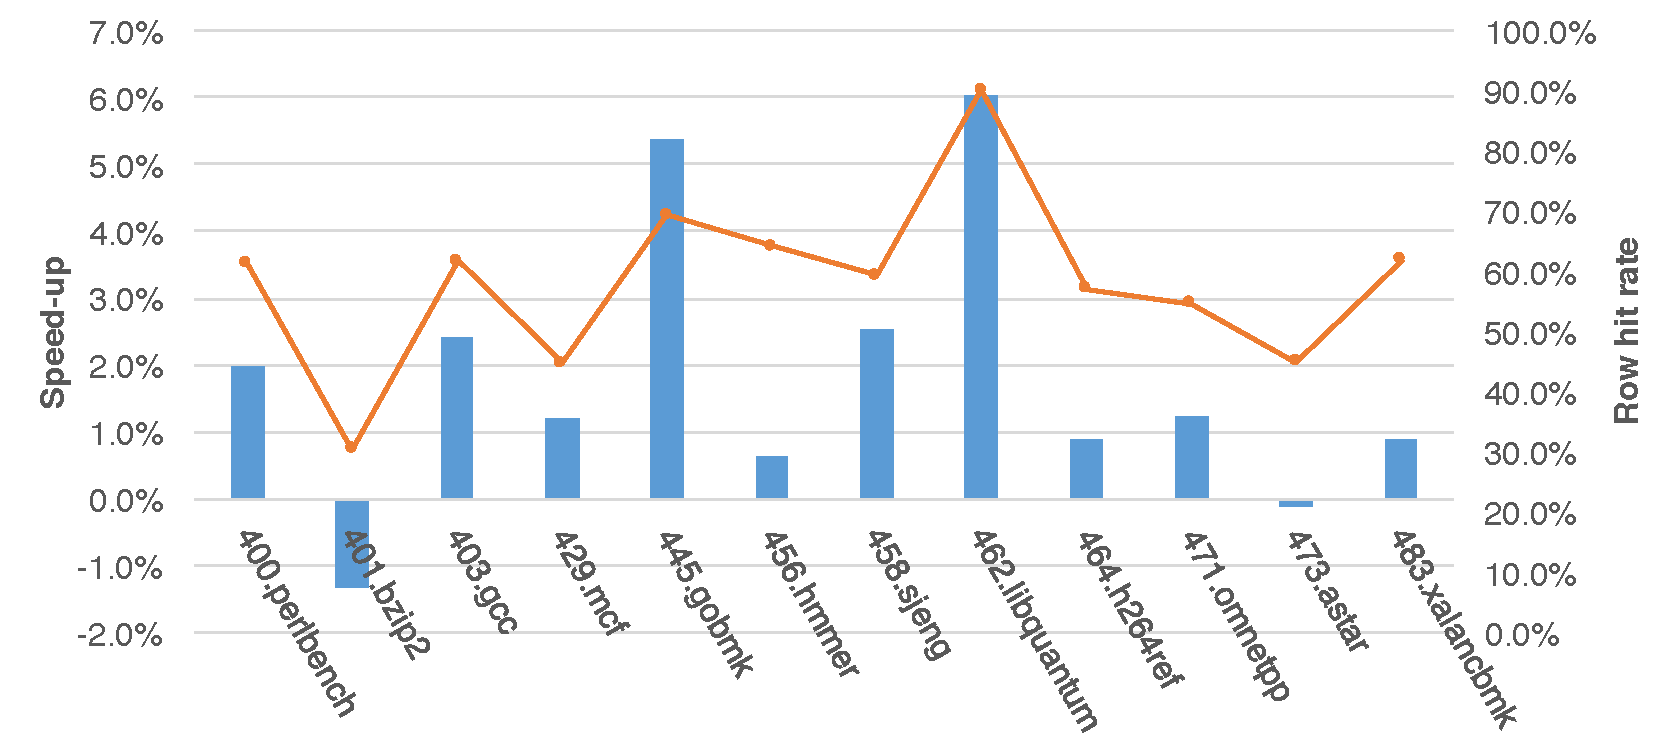
\includegraphics[width=\columnwidth]{figures/rocket-fifomas.pdf}
		\caption{Speedup of the open-page FCFS MAS policy over the close-page policy for Rocket}
		\label{fig:rocket_fifo_mas}
\end{figure}

This section shows the performance impacts of the page policies with the FCFS MAS model
(Section~\ref{sec:timing_model}). This represents a more complex policy, and we contrast variants with open and close row policies.

\begin{table}[t]
\centering
\resizebox{0.5\textwidth}{!}{%
\begin{tabular}{|c|c c|}
\hline
\textbf{Parameter} & \textbf{Open Policy} & \textbf{Close Policy} \\
\hline
\textit{number of banks} & 8 & 8 \\
\textit{bank address offset} & \textbf{13} & \textbf{6} \\
\textit{row address offsets} & 16 & 16 \\
\textit{bandwidth} & 8 & 8 \\
\textit{tRC} & 7 cycles & 7 cycles \\
\textit{tRCD} & 7 cycles & 7 cycles\\
\textit{tCAS} & 7 cycles & 7 cycles \\
\hline
\end{tabular}}
\caption{FIFO MAS Parameters}
\label{tbl:fifo_mas}
\end{table}

Table~\ref{tbl:fifo_mas} lists the parameter values used in this experiment.
Figure~\ref{fig:rocket_fifo_mas} shows the speedup of the open page policy over
the close page policy for the SPEC benchmarks and the DaCapo benchmarks running
on Rocket, along with the row hit rate for each benchmark. Overall, the open
page policy has perfomance benefits for the SPEC CPU integer benchmarks except
for \textit{402.bzip2} and \textit{473.astar}. As indicated in
Figure~\ref{fig:rocket_fifo_mas}, the memory requests of \textit{402.bzip2} and
\textit{473.astar} lack locality (resulting in low row hit rates), which
explains these results.
